\documentclass[red]{tutorial}
\usepackage[no-math]{fontspec}
\usepackage{xpatch}
	\renewcommand{\ttdefault}{ul9}
	\xpatchcmd{\ttfamily}{\selectfont}{\fontencoding{T1}\selectfont}{}{}
	\DeclareTextCommand{\nobreakspace}{T1}{\leavevmode\nobreak\ }
\usepackage{polyglossia} % English please
	\setdefaultlanguage[variant=us]{english}
%\usepackage[charter,cal=cmcal]{mathdesign} %different font
%\usepackage{avant}
\usepackage{microtype} % Less badboxes

%\usepackage{enumitem}

\usepackage[charter,cal=cmcal]{mathdesign} %different font
%\usepackage{euler}
 
\usepackage{blindtext}
\usepackage{calc, ifthen, xparse, xspace}
\usepackage{makeidx}
\usepackage[hidelinks, urlcolor=blue]{hyperref}   % Internal hyperlinks
\usepackage{mathtools} % replaces amsmath
% \usepackage{amsmath}
\usepackage{bbm} %lower case blackboard font
\usepackage{amsthm, bm}
\usepackage{thmtools} % be able to repeat a theorem
\usepackage{thm-restate}
\usepackage{graphicx}
\usepackage{multicol}
\usepackage{fnpct} % fancy footnote spacing
\usepackage{tikz}
\usetikzlibrary{arrows.meta}
\newcommand{\checkbox}{\tikz[baseline=-1mm,line width=1]{\draw (0,0) circle (0.15);}}
\definecolor{tolOrange}{HTML}{EE7733} 
\usepackage{tcolorbox}
\definecolor{tolBlue}{HTML}{0077BB}
\definecolor{tolCyan}{HTML}{33BBEE}
\definecolor{tolTeal}{HTML}{009988} 
\definecolor{tolOrange}{HTML}{EE7733} 
\definecolor{tolRed}{HTML}{CC3311} 
\definecolor{tolMagenta}{HTML}{EE3377} 
\definecolor{tolGrey}{HTML}{BBBBBB}
\usepackage{enumitem}

\usepackage{pgfplots}
\pgfplotsset{compat=1.18}
%\pgfkeys{/pgf/fpu}

 
\newcommand{\xh}{{{\mathbf e}_1}}
\newcommand{\yh}{{{\mathbf e}_2}}
\newcommand{\zh}{{{\mathbf e}_3}}
\newcommand{\R}{\mathbb{R}}
\newcommand{\Z}{\mathbb{Z}}
\newcommand{\N}{\mathbb{N}}
\newcommand{\proj}{\mathrm{proj}}
\newcommand{\Proj}{\mathrm{proj}}
\newcommand{\Perp}{\mathrm{perp}}
\renewcommand{\span}{\mathrm{span}\,}
\newcommand{\Span}{\mathrm{span}\,}
\newcommand{\Img}{\mathrm{img}\,}
\newcommand{\Null}{\mathrm{null}\,}
\newcommand{\Range}{\mathrm{range}\,}
\newcommand{\rref}{\mathrm{rref}}
\newcommand{\rank}{\mathrm{rank}}
\newcommand{\Rank}{\mathrm{rank}}
\newcommand{\nnul}{\mathrm{nullity}}
\newcommand{\mat}[1]{\begin{bmatrix}#1\end{bmatrix}}
\newcommand{\chr}{\mathrm{char}}
\renewcommand{\d}{\mathrm{d}}


\theoremstyle{definition}
\newtheorem{example}{Example}[section]
\newtheorem{defn}{Definition}[section]

%\theoremstyle{theorem}
\newtheorem{thm}{Theorem}[section]

\pgfkeys{/tutorial,
	name={Tutorial 7},
	author={},
	course={MAT 187},
	date={},
	term={},
	title={Introduction to Ordinary Differential Equations}
	}

\begin{document}
	\begin{tutorial}
		\begin{objectives}
	In this tutorial you will characterize first order differential equations.
\end{objectives}

\subsection*{Problems}
\begin{enumerate}
\item Draw a phase plot (plot of $y$ vs., $f(y)$) for an autonomous ODE $y'=f(y)$ such that:
\begin{itemize}[nosep]
	\item The ODE has three equilibria.
	\item At least one of the equilibria is stable.
	\item \textbf{NONE} of the equilibria are unstable.
\end{itemize}
Explain and justify that your phase plot does actually fulfill these requirements.

\item Consider the following ODEs. Are they linear or not? Are they separable or not?
\begin{tcolorbox}[sharp corners=all,colframe=tolGrey,colback=white]
    \begin{multicols}{2}
    \begin{enumerate}[label={(\roman{enumii})},nosep,itemsep=1mm]
        \item $y'=t^2y$
        \item $y'=t\sin y$
        \item $y'=y\sin t$
        \item $y'=t+\sin y$
        \item $y'=y+\sin t$
        \item $y'=y(t^2+1)$
        \item $y'=e^{2t-y}$
        \item $y'-2y=3e^t$
        \item $y'e^{t/2}=y^2+4$
        \item $y'+y=5\sin 2t$
    \end{enumerate}
    \end{multicols}
\end{tcolorbox}

\item Consider the below ODES and problem descriptions. Match each ODE to a problem description and justify your answer.
\begin{tcolorbox}[sharp corners=all,colframe=tolGrey,colback=white]
    \begin{multicols}{2}
    \begin{enumerate}[label={(\roman{enumii})},nosep,itemsep=1mm]
        \item $y'=ky$
        \item $y'=ky(M-y)$
        \item $y'=\frac{ky(M-y)}{\sqrt{t+1}}$
    \end{enumerate}
    \end{multicols}
\end{tcolorbox}

Consider the below descriptions:
\begin{enumerate}
    \item Babies are born on an island at a constant rate, but there is a carrying capacity which limits the number of people that the island can support.
    \item Babies are born on an island at a constant rate.
    \item Babies are born on an island at a constant rate, but as time progresses, people become more rich and have fewer children.
\end{enumerate}

% \begin{minipage}[t]{\linewidth-7cm}
% \item Consider the ODE
% \[
%     \frac{\mathrm dy}{\mathrm dt} = f(y) = (y-1)^2 (y-2) (y-3)
% \]
% The phase plot of this ODE is given on the right.

% \textit{You can answer this question based on the equation, the phase plot, or both!}
% \begin{enumerate}
% \item Find and classify the equilibrium points of the differential equation. Make sure to justify your answer.
% \vspace{3mm}

% \item If $y(t)$ is a solution to the ODE, and $y(0.5)=2.8$, what is $\lim_{t\to\infty} y(t)$? Justify your choice.
% \end{enumerate}
% \end{minipage}\hfill
% \begin{minipage}[t]{6cm}
% 	\vfil
% 	\vspace{-6mm}
% 	\flushright
% 	\begin{tikzpicture}[line width=1]
% 		\draw [black!20] (-0.5,-1) grid [step=0.5] (4,3);
% 		\begin{scope}
% 		\clip (0,-1) rectangle (4,3);
% 		\draw [smooth,samples=100,domain=0:3.5,tolOrange] plot ({\x},{(\x-1)*(\x-1)*(\x-2)*(\x-3)});
% 		\end{scope}
% 	\draw [->] (-0.5,0) -- (4,0) node [right] {$y$};
% 	\draw [->] (0,-1) -- (0,3) node [above] {$f(y)$};
% 	\draw (1,0.1) -- (1,-0.1) node [below] {1};
% %	\draw (0.1,1) -- (-0.1,1) node [left] {1};
% \end{tikzpicture}
% \end{minipage}

% \clearpage
% \item Match the direction fields below with the following ODEs. There are more ODEs than figures, so some won't have a match. Make sure to provide an argument in words justifying the matching.
% \begin{multicols}{2}
%     \begin{enumerate}[label={(\roman{enumii})},nosep,itemsep=1mm]
%         \item $y'=2y-1$
%         \item $y'=2+y$
%         \item $y'=y-2$
%         \item $y'=y(y+3)$
%         \item $y'=y(y-3)$
%         \item $y'=1+2y$
%         \item $y'=-2-y$
%         \item $y'=y(3-y)$
%         \item $y'=1-2y$
%         \item $y'=2-y$
%     \end{enumerate}
%     \end{multicols}

% 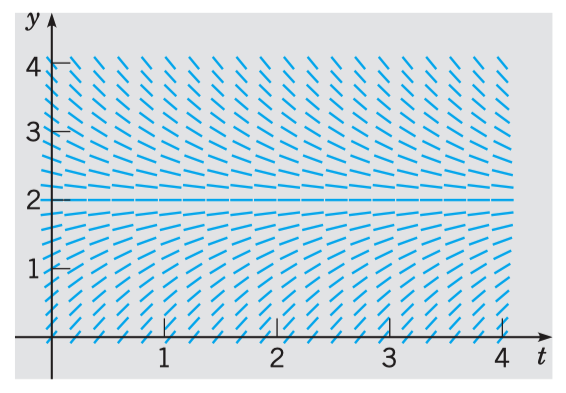
\includegraphics[width=0.4\linewidth]{field1}
% 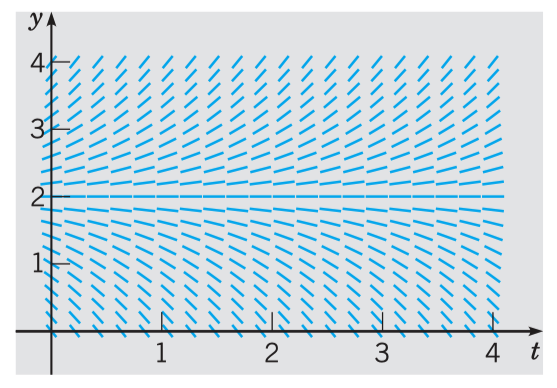
\includegraphics[width=0.4\linewidth]{field2}\\
% \null\hfill\textbf{(A)}\hfill\hfill
% \textbf{(B)}\hfill
% \null

% \vspace{3mm}
% \hrule

% 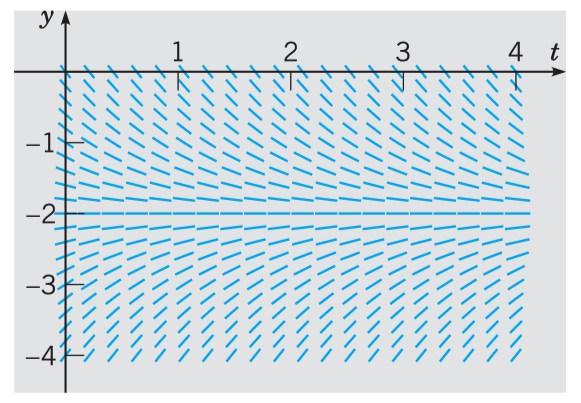
\includegraphics[width=0.4\linewidth]{field3}
% 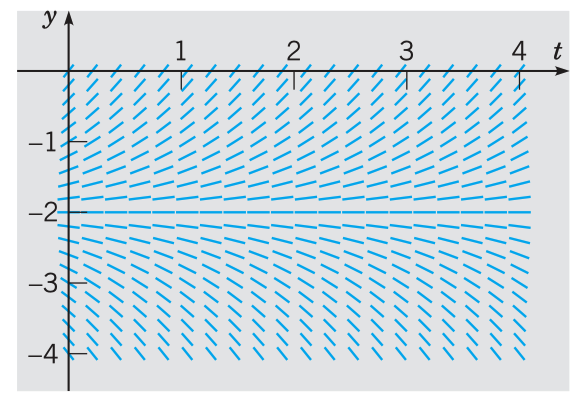
\includegraphics[width=0.4\linewidth]{field4}\\
% \null\hfill\textbf{(C)}\hfill\hfill
% \textbf{(D)}\hfill
% \null

% \vspace{3mm}
% \hrule

% 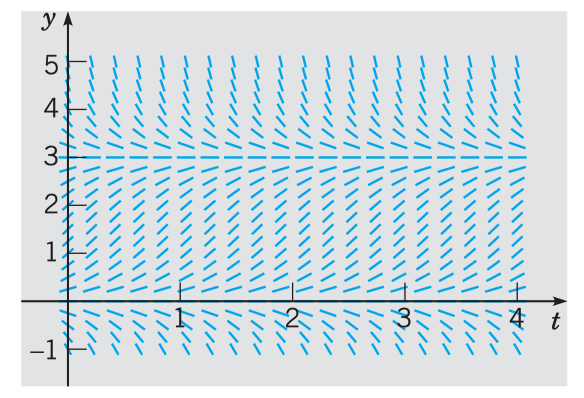
\includegraphics[width=0.4\linewidth]{field5}
% 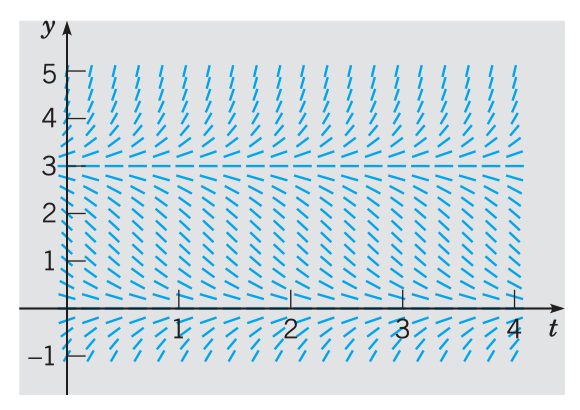
\includegraphics[width=0.4\linewidth]{field6}\\
% \null\hfill\textbf{(E)}\hfill\hfill
% \textbf{(F)}\hfill
% \null
% \clearpage

% \item We will attempt to model how people leave a soccer stadium at the end of a game. We define the radius of the populated area in the stadium around an exit as $r(t)$. $t$ is the time in minutes and our observation starts at $t=0$.
	
% 	The flow of people will obey Torricelli’s Law which states that \textit{the area of the region occupied by people will decrease at a rate proportional to the square root of the radius and also proportional to the size of the exit}.
	
% 	\begin{enumerate}
% 	\begin{minipage}[t]{0.50\linewidth} 
%     	\item Use this to create an ODE that models the size of the crowd exiting the stadium. Introduce parameters as necessary.\medskip
    	
%     	\item Classify the ODE from the last part (order, linearity, separability etc.). Without solving the ODE, consider each parameter and each variable: What are its units? How does it affect the behaviour of the ODE? How is the behaviour of this system affected if it is very large? very small? zero?\medskip

        
        
%         \item Find the general solution to the ODE. What is the solution if $r(0)=3$?
%     	\end{minipage}\hfill
%     	\begin{minipage}[t]{0.33\textwidth} 
%     	\vfil
%             \begin{flushright}
%             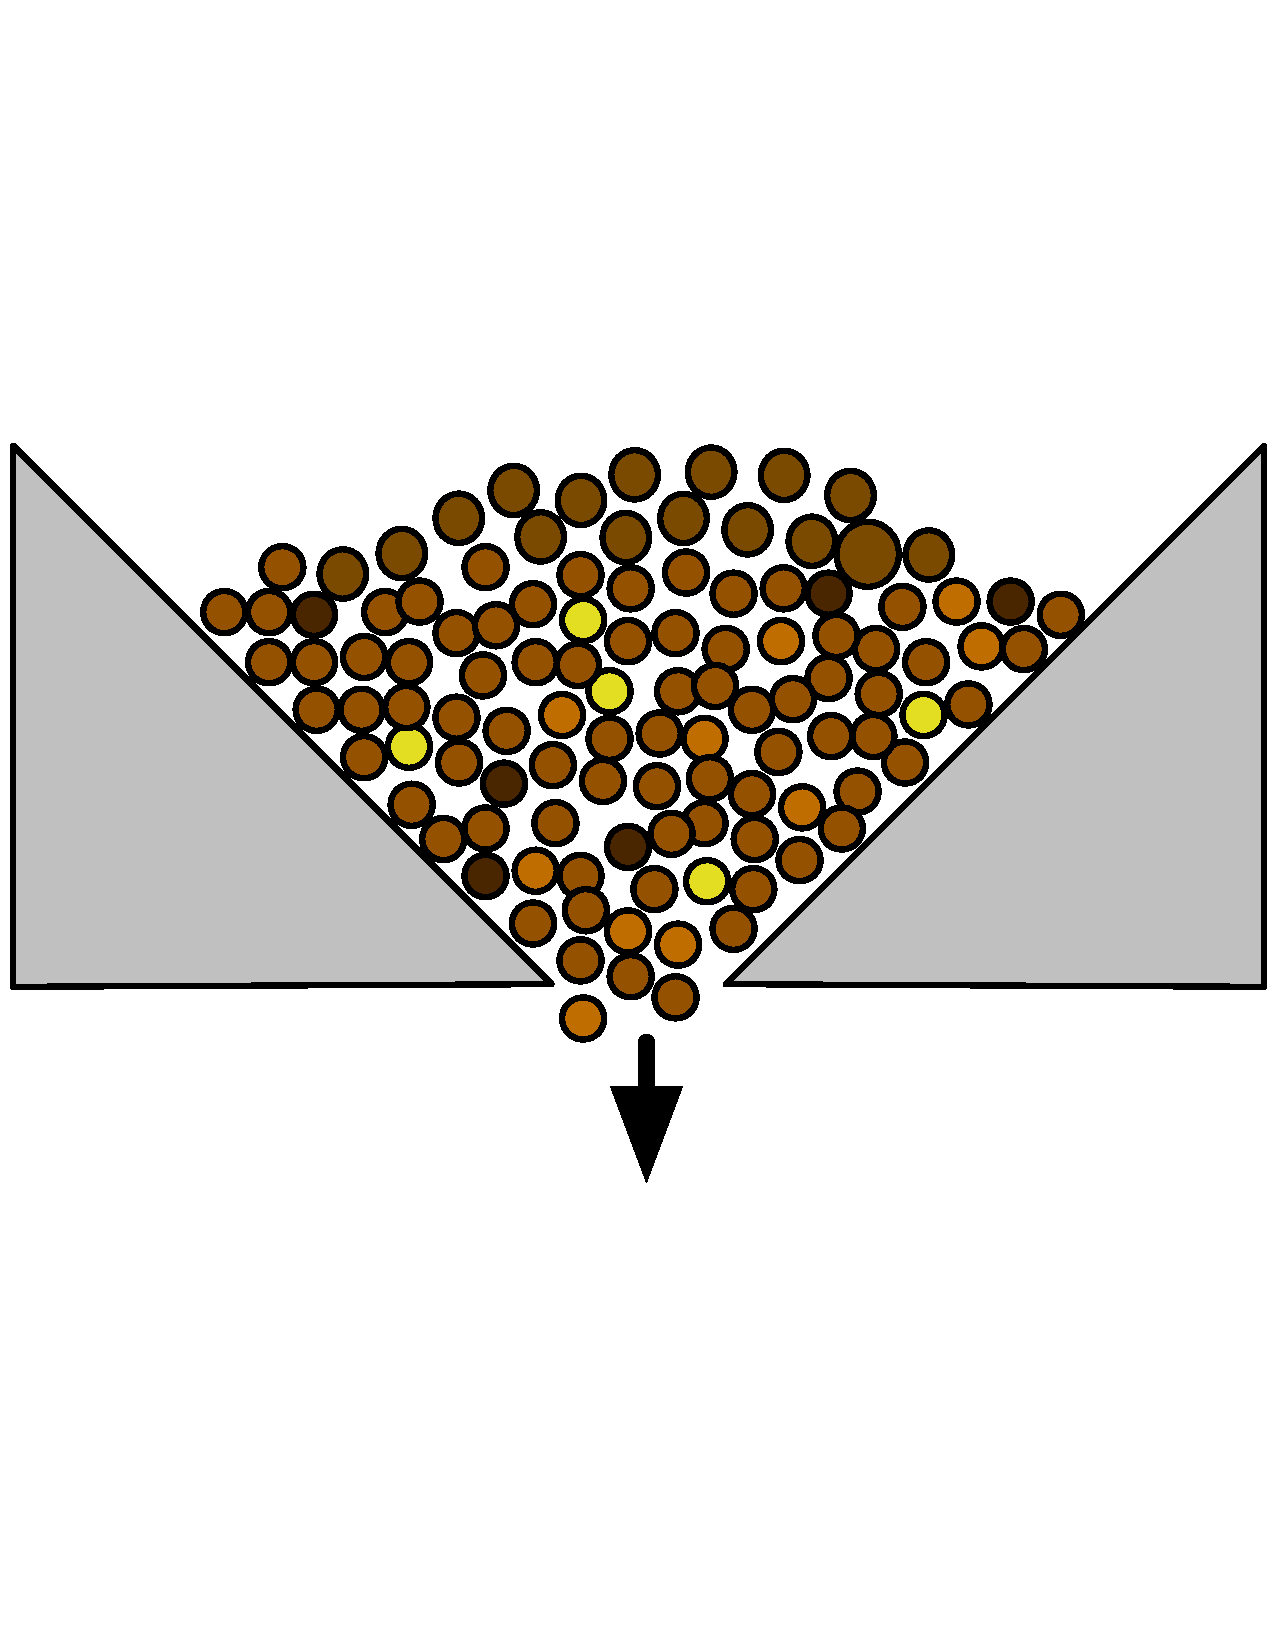
\includegraphics[width=1.0\textwidth]{stadium_fixed.pdf}\\
%             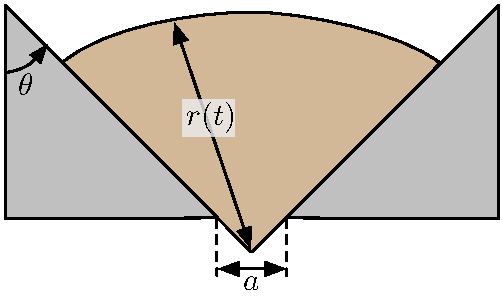
\includegraphics[width=1.0\textwidth]{stadium2.pdf}    
%             \end{flushright}
%         \end{minipage}
%     \end{enumerate}
\end{enumerate}

	\end{tutorial}

	\begin{solutions}
		\begin{enumerate}
    \item 

        \begin{enumerate}
        \begin{enumerate}
            \item Linear, separable
            \item Nonlinear, separable
            \item Linear, separable
            \item Nonlinear, nonseparable
            \item Linear, nonseparable
            \item Linear, separable
            \item Nonlinear, separable
            \item Linear, nonseparable
            \item Nonlinear, separable
            \item Linear, nonseparable
            
        \end{enumerate}
        \end{enumerate} 
    \item 
    $y=1$ is semistable,
    $y=2$ is stable,
    $y=3$ is unstable
    
    A visual argument (``If we are just below 1, the derivative is positive, so it's going back to 1'') is nicer than an abstract argument that seems memorized (``If the phase plot crosses from top left to bottom right, it is stable'')

    \item 
    We first note that all ODEs are first-order and autonomous, meaning we can look at their roots to find their equilibrium points and match them with the given direction fields. 
    
    Direction field (A) shows one equilibrium solution at $y = 2$. Therefore, either $y' = y - 2$ or $y'= 2 - y$ are valid candidates. We also see that for $y > 2$, the solutions are decreasing (i.e., $y' < 0$) while for $y < 2$, the solutions are increasing (i.e., $y' > 0$). Therefore, $y' = 2 - y$ must be the matching ODE.
    
    A similar line of reasoning applies for direction field (B) where now we see that for $y > 2$, the solutions are increasing (i.e., $y' > 0$) while for $y < 2$, the solutions are decreasing (i.e., $y' < 0$). Therefore, $y' = y - 2$ must be the matching ODE.
    
    Matching direction fields (C) and (D) follows a similar line of reasoning as matching direction fields (A) and (B). The only difference is that the equilibrium point is at $y = -2$, meaning either $y' = 2 + y$ or $y' = -2-y$ are valid ODEs. For direction field (C), $y' < 0$ for $y > -2$ and $y' > 0$ for $y < -2$. Therefore, $y' = -2 - y$ is the matching ODE. This leaves direction field (D) to match $y' = 2 + y$.
    
    Direction fields (E) and (F) have equilibrium points at $y = 0$ and $y = 3$, meaning $y' = y(3-y)$ and $y' = y(y-3)$ are potential candidates. For direction field (E), $y' < 0$ for $y < 0, y > 3$ and $y' > 0$ for $0 < y < 3$. Therefore, $y' = y(3 - y)$ is the matching ODE. This leaves direction field (F) to match $y' = y(y-3)$.
\end{enumerate}
	
	\end{solutions}
	\begin{instructions}
		\subsection*{Learning Objectives}
Students need to be able to\ldots
\begin{itemize}
	\item  
\end{itemize}

\subsection*{Context}

\subsection*{Notes}
\begin{enumerate}
	\item This question should be a good warmup to the tutorial. 
\end{enumerate}
	\end{instructions}

\end{document}
